\subsection{Evaluation of Considered Scheduling Algorithms}\label{sec:application:cloud_file_synchronisation:numerical_evaluation}
In order to evaluate the proposed model we use the OMNeT++\footnote{\url{http://www.omnetpp.org/}, \accessed} simulation framework.
To analyse the impact of the different algorithms we study the metrics introduced in \refsec{sec:application:cloud_file_synchronisation:system_model}.
We evaluate the waiting time \sojournTime until a file is retrieved at the downloading client, the relative time the mobile client stays disconnected \relativeDisconnectedTime during the synchronisation process, and the number of connection \connectionCount during the synchronisation process to estimate the signalling overhead.
For the \algointerval scheduling algorithm, we vary the interval length \thresholdInterval from \SI{1}{\second} to \SI{512}{\second} in powers of two.
The threshold \thresholdSize for the \algosize algorithm is analysed for values from \SI{1}{\mega\byte} to \SI{512}{\mega\byte} in the same manner.
The \algoimmediate algorithm is not parametrised.

In the simulated scenario, we assume a user synchronising \(\numberOfFiles = 1000\) files from the camera to the downloading client.
For each parameter set we perform \(100\) repetitions.

\subsubsection*{Waiting Time}\label{sec:application:cloud_file_synchronisation:numerical_evaluation:waiting_time}
First, we analyse the mean waiting time \sojournTime required to transfer a picture from the camera to the wire-lined download client for the different scheduling algorithms and different parameter sets.
The mean waiting times \sojournTime and the corresponding \SI{95}{\percent} confidence intervals are shown in \reffig{fig:application:cloud_file_synchronisation:numerical_evaluation:waiting_time:waiting_time}.
For most of the derived mean values, the confidence intervals are not visible due to their small size.

\begin{figure}
	\begin{subfigure}[b]{\textwidth}
	\centering
	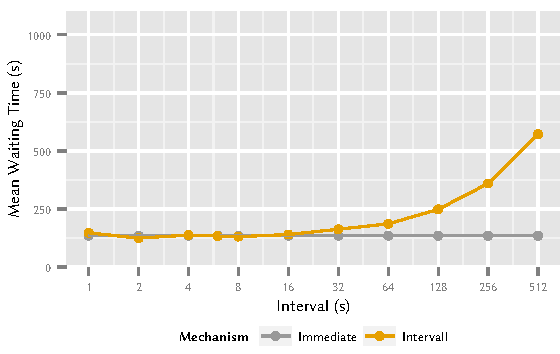
\includegraphics{application/cloud_file_synchronization/numerical_evaluation/figures/interval_delay}
	\caption{Algorithm \algointerval, different interval lengths \thresholdInterval}\label{fig:application:cloud_file_synchronisation:numerical_evaluation:waiting_time:waiting_time:interval}
	\end{subfigure} 
	\begin{subfigure}[b]{\textwidth}
	\centering
	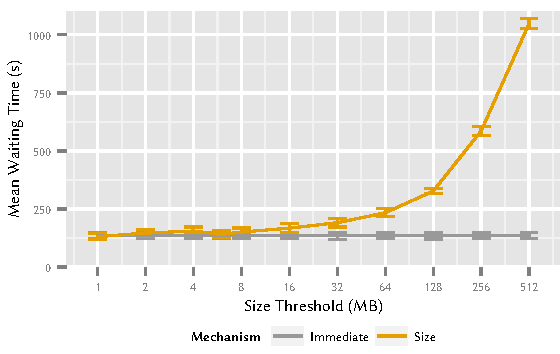
\includegraphics{application/cloud_file_synchronization/numerical_evaluation/figures/size_delay}
	\caption{Algorithm \algosize, different threshold sizes \thresholdSize}\label{fig:application:cloud_file_synchronisation:numerical_evaluation:waiting_time:waiting_time:size}
	\end{subfigure}

	\caption{Comparison of algorithms with regard to waiting time \sojournTime.}\label{fig:application:cloud_file_synchronisation:numerical_evaluation:waiting_time:waiting_time}
\end{figure}

\reffig{fig:application:cloud_file_synchronisation:numerical_evaluation:waiting_time:waiting_time:interval} shows the results for the \algointerval algorithm, \reffig{fig:application:cloud_file_synchronisation:numerical_evaluation:waiting_time:waiting_time:size} shows the results for the \algosize mechanisms. 
In \reffig{fig:application:cloud_file_synchronisation:numerical_evaluation:waiting_time:waiting_time:interval} the x-axis shows the length of the interval \thresholdInterval in \si{\second} between sending newly added files, in \reffig{fig:application:cloud_file_synchronisation:numerical_evaluation:waiting_time:waiting_time:size} the axis shows the required cumulated size in \si{\mega\byte} of new files before an upload is triggered.
The y-axis in both figures show the mean waiting time \sojournTime in \si{\second}.
The result of the \algoimmediate algorithm is added in both figures as a reference.
Note, the mean waiting time \sojournTime for this algorithms is independent of the parameters used for the other two algorithms, as files are always uploaded immediately after they have been copied to the \dropbox folder.

\reffig{fig:application:cloud_file_synchronisation:numerical_evaluation:waiting_time:waiting_time:interval} shows that the mean waiting time \sojournTime depends on the interval length \thresholdInterval of the \algointerval algorithm. 
For interval lengths \thresholdInterval smaller than \SI{8}{\second}, the waiting times do not differ significantly from the mean waiting times \sojournTime obtained by the \algoimmediate algorithm.
This can be explained by the average file size of \SI{3.5}{\mega\byte} of the images and the assumed average Bluetooth transmission rate of \SI{0.5}{\mega\bit\per\second}, which results in an average inter arrival time of \SI{7}{\second}.
For interval lengths \thresholdInterval less than \SI{7}{\second}, there is almost always an image in the upload queue so that the algorithm performs similar to the \algoimmediate strategy. 
For interval lengths \thresholdInterval larger than \SI{7}{\second}, the average waiting time increases for the \algointerval algorithm.
Here, the files are already preprocessed and accumulate in the uploading queue until the next batch upload starts resulting in an increased mean waiting time \sojournTime.
For very large values of the interval lengths \thresholdInterval, the mean waiting time \sojournTime is dominated by the interval length \thresholdInterval.
This mean that the mobile client's mean waiting time \sojournTime before starting the upload is much longer that the upload duration of the images.
Thus, the mean waiting time \sojournTime converges to the interval length \thresholdInterval for extreme values.

\reffig{fig:application:cloud_file_synchronisation:numerical_evaluation:waiting_time:waiting_time:size} depicts the mean waiting time \sojournTime for the \algosize algorithms for different file size thresholds \thresholdSize.
We observer that for values smaller than the average image file size of \SI{3.5}{\mega\byte}, the \algosize algorithms performs similar to the \algoimmediate algorithms.
In this case the \algosize algorithms also triggers an upload for almost each file and shows the same behaviour as the \algoimmediate algorithm.
For size thresholds \thresholdSize smaller than \SI{16}{\mega\byte}, the performance of the \algosize algorithms is only slightly worse than the reference mechanism.
Here, only a few files are required to trigger the upload process and the additional delay introduced by waiting is negligible.
For larger size thresholds \thresholdSize, the mean waiting time \sojournTime increases significantly.

\subsubsection*{Relative Disconnection Time}\label{sec:application:cloud_file_synchronisation:numerical_evaluation:relative_disconnection_time}

Besides a fast synchronisation, the users also demand a long battery life time of the mobile device.
Besides the display, the radio interface used to establish Internet connection is one of the main power consumers.
In order to analyse the power savings of the different algorithms, we evaluate the relative disconnected time  \relativeDisconnectedTime during the synchronisation process.
Therefore, we consider the time between the sending of the first and the last image of the mobile client and calculate the percentage during which no Internet connection is established.
The mean relative disconnected times including the \SI{95}{\percent} confidence intervals are depicted in \reffig{fig:application:cloud_file_synchronisation:numerical_evaluation:disconnected:disconnected}. 

\begin{figure}
	\begin{subfigure}[b]{\textwidth}
	\centering
	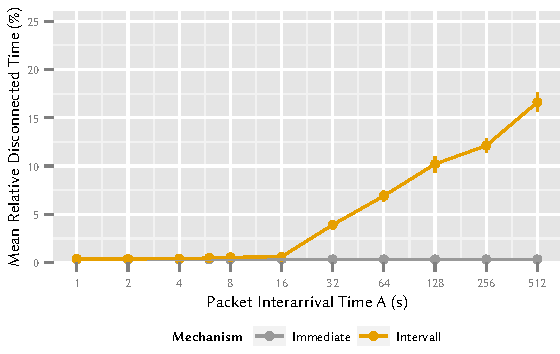
\includegraphics{application/cloud_file_synchronization/numerical_evaluation/figures/interval_disconnected}
	\caption{Algorithm \algointerval, different interval lengths \thresholdInterval}\label{fig:application:cloud_file_synchronisation:numerical_evaluation:disconnected:disconnected:interval}
	\end{subfigure} 
	\begin{subfigure}[b]{\textwidth}
	\centering
	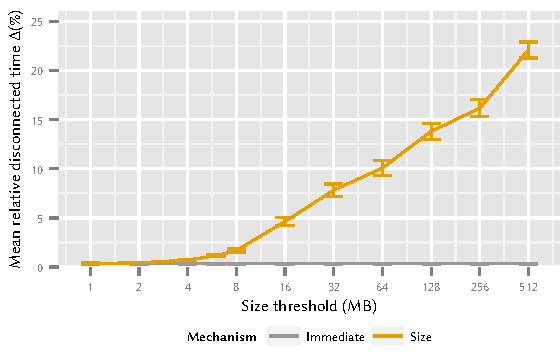
\includegraphics{application/cloud_file_synchronization/numerical_evaluation/figures/size_disconnected}
	\caption{Algorithm \algosize, different threshold sizes \thresholdSize}\label{fig:application:cloud_file_synchronisation:numerical_evaluation:disconnected:disconnected:size}
	\end{subfigure}

	\caption{Comparison of algorithms with regard to relative disconnected time \relativeDisconnectedTime.}\label{fig:application:cloud_file_synchronisation:numerical_evaluation:disconnected:disconnected}
\end{figure}

\reffig{fig:application:cloud_file_synchronisation:numerical_evaluation:disconnected:disconnected:interval} depicts the relative disconnected time \relativeDisconnectedTime on the y-axis, on the x-axis the interval length \thresholdInterval in \si{\second} for the \algointerval algorithm. 
\reffig{fig:application:cloud_file_synchronisation:numerical_evaluation:disconnected:disconnected:size} also depicts the relative disconnected time \relativeDisconnectedTime on the y-axis, on the x-axis the size threshold \thresholdSize in \si{\mega\byte} for the \algosize algorithm. 
Both figures include the \algoimmediate algorithm as a reference.

We first study \reffig{fig:application:cloud_file_synchronisation:numerical_evaluation:disconnected:disconnected:interval}.
Similar to \reffig{fig:application:cloud_file_synchronisation:numerical_evaluation:waiting_time:waiting_time:interval}, we observe no significant differences between the \algointerval and \algoimmediate algorithm for interval lengths \thresholdInterval smaller than \SI{8}{\second}, as both algorithms show the same behaviour here.
For values larger than \SI{8}{\second}, the \algointerval algorithm starts sending files in batches and no longer on a per file base.
However, still no clear effect is visible, as the inter-sending interval and the mean image inter-arrival time of files is still smaller than the disconnection timeout of \SI{11}{\second}.
This results in an almost permanent Internet connection similar to the \algoimmediate algorithm.
For interval lengths \thresholdInterval above \SI{16}{\second}, the \algointerval algorithm starts saving connection time and the relative disconnected time \relativeDisconnectedTime increases, resulting in additional power savings.

\reffig{fig:application:cloud_file_synchronisation:numerical_evaluation:disconnected:disconnected:size} shows the relative disconnected time \relativeDisconnectedTime for variable thresholds for the \algosize algorithm.
We see again that the \algosize and \algoimmediate algorithms do not differ for size thresholds \thresholdSize smaller than \SI{4}{\mega\byte}, similar to the results in \reffig{fig:application:cloud_file_synchronisation:numerical_evaluation:waiting_time:waiting_time:size}.
Afterwards, we observe an increase in saved relative connection time \relativeDisconnectedTime for larger thresholds \thresholdSize, due to the fact that here files are sent in batches and the mobile client disconnects between the sending intervals, again enabling power saving potential for the mobile network client.

\subsubsection*{Connection Count}\label{sec:application:cloud_file_synchronisation:numerical_evaluation:connection_count}

After considering the requirements of the end-user, we have a closer look at the requirements of the mobile network operators.
The network operator is mainly interested in minimising the signalling overhead introduce by connection establishment.
Therefore, a minimisation of the number of connections \connectionCount during the synchronisation process is desired.
\reffig{fig:application:cloud_file_synchronisation:numerical_evaluation:connection:connection} depicts the average number of connections \connectionCount established during the synchronisation process, including the 95\% confidence intervals.
The number of connections is shown on the y-axis, the x-axis in \reffig{fig:application:cloud_file_synchronisation:numerical_evaluation:connection:connection:interval} shows the interval lengths \thresholdInterval of the \algointerval algorithms, the x-axis in \reffig{fig:application:cloud_file_synchronisation:numerical_evaluation:connection:connection:size} shows the \algosize algorithm size threshold \thresholdSize.

\begin{figure}
	\begin{subfigure}[b]{\textwidth}
	\centering
	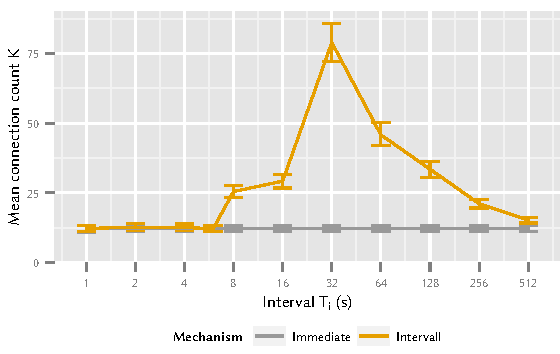
\includegraphics{application/cloud_file_synchronization/numerical_evaluation/figures/interval_connection}
	\caption{Algorithm \algointerval, different interval lengths \thresholdInterval}\label{fig:application:cloud_file_synchronisation:numerical_evaluation:connection:connection:interval}
	\end{subfigure} 
	\begin{subfigure}[b]{\textwidth}
	\centering
	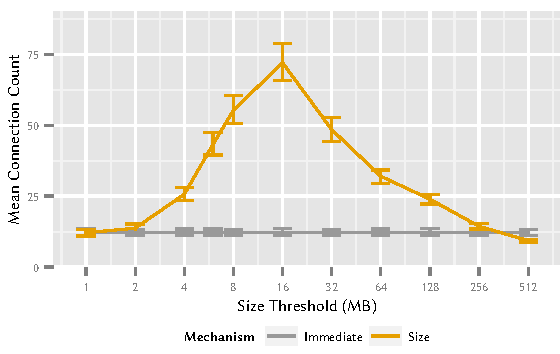
\includegraphics{application/cloud_file_synchronization/numerical_evaluation/figures/size_connection}
	\caption{Algorithm \algosize, different threshold sizes \thresholdSize}\label{fig:application:cloud_file_synchronisation:numerical_evaluation:connection:connection:size}
	\end{subfigure}

	\caption{Comparison of algorithms with regard to connection count \connectionCount.}\label{fig:application:cloud_file_synchronisation:numerical_evaluation:connection:connection}
\end{figure}

We observer a similar behaviour as in the previous evaluations, the average number of connection \connectionCount for the \algointerval and the \algoimmediate algorithms is the same in \reffig{fig:application:cloud_file_synchronisation:numerical_evaluation:connection:connection:interval}, if the interval lengths \thresholdInterval are smaller then \SI{4}{\second}.
With increasing interval lengths \thresholdInterval the connection count \connectionCount also increases and reaches a maximum for an interval length of \SI{32}{\second}.

%TODO: check SI containing variables
In order to explain this behaviour we make the following considerations.
The maximum amount of data \(s_x\) which can be send from the camera to the mobile client during an intervals \thresholdInterval of length \(x~\si{\second}\) is given by 
\[s_x=x \cdot \panTransferRate = x \cdot \SI{1 / 2}{\mega\byte}.\]
The average time \(t_x\) to upload \(s_x\) can now be calculated as 
\[t_x = s_x / E\left[\uploadbandwidth\right] = x~\SI{0.5 / 8.0}{\second} = x~\SI{1 / 16}{\second}.\]
For interval lengths \thresholdInterval between \SI{8}{\second} and \SI{32}{\second}, \(t_x\) results in \SI{0.5}{\second}, \SI{1}{\second}, and \SI{2}{\second} respectively.
Considering the disconnection timeout of \SI{11}{\second}, we can see that a disconnect is likely for interval lengths \thresholdInterval of \SI{16}{\second} and \SI{32}{\second}.
In order to explain the increased number of connections \connectionCount for an interval length \thresholdInterval of \SI{8}{\second}, we also have to consider the average image file size of \SI{3.5}{\mega\byte}.
Within \SI{8}{\second}, a maximum of \(s_x = \SI{4}{\mega\byte}\) can be transferred from the camera to the mobile client.
Therefore, it is likely that it takes two interval lengths \thresholdInterval, respectively \SI{16}{\second}, to transfer the image.
This explains the similar behaviour of the \algointerval algorithm for interval lengths \thresholdInterval between \SI{8}{\second} and \SI{16}{\second} with regard to the connection count \connectionCount.

For interval lengths \thresholdInterval larger then \SI{32}{\second}, the connection count \connectionCount decreases again.
To explain this effect, we have to consider the maximum number of file batches transferred during the synchronisation process.
If every file is transferred individually \(1000\) connections would be required, if all files are transferred in one single batch, only one connection would be established during the synchronisation process.
Depending on the chosen interval lengths \thresholdInterval, the average sizes of the batches varies, as larger intervals result in larger batches.
The overall number of batches is limited, as we only consider a finite amount of \(1000\) images.
Consequently, the maximum possible number of connections \connectionCount is limited, too.
However, this comes only into effect if large batches are used during the synchronisation process.

In \reffig{fig:application:cloud_file_synchronisation:numerical_evaluation:connection:connection:size} we can observe similar behaviours of the \algosize algorithm as for the \algointerval algorithm in \reffig{fig:application:cloud_file_synchronisation:numerical_evaluation:connection:connection:interval}.
For small thresholds, the \algosize and the \algoimmediate algorithm result in the same number of connections \connectionCount .
With increasing sending thresholds, the number of disconnects and re-connections increases, as it takes longer to accumulate the required amount of new data at the mobile client.
The maximum average connection count \connectionCount is reached when using a \SI{16}{\mega\byte} threshold, which corresponds to \(s_x\) for an inter-sending interval of \SI{32}{\second}.
For larger thresholds, the maximum number of batches is the limiting factor for the connection count.
This can especially be observed for very large thresholds.
Considering a size threshold \thresholdSize of \SI{128}{\mega\byte}, we can assume that almost every batch is transferred in an individual connection, as it takes \(\SI{128}{\mega\byte} / \panTransferRate = \SI{248}{\second}\) to transfer the required data from the camera to the mobile client, but only \(\SI{128}{\mega\byte} / E\left[\uploadbandwidth\right] = \SI{16}{\second}\) on average to upload the data from the mobile client to the cloud.
Consequently, the transferred file size can be estimated as the product of the size threshold \thresholdSize and number of connections, i.e. \(\SI{128}{\mega\byte} \cdot 25 = \SI{3.2}{\giga\byte}\), which approximately matches the product of number of considered files and the average file size.

\subsubsection*{Mechanism Comparison}\label{sec:application:cloud_file_synchronisation:numerical_evaluation:mechanism_comparison}
The previous analyses imply that the results of the \algointerval and \algosize algorithm are interchangeable if the parameters are set appropriately.
In order to test this hypothesis, we normalise the size threshold parameter \thresholdSize with the \gls{PAN} bandwidth to calculate the effective average interval length caused by this threshold.
The mean connection count \connectionCount for both algorithms depending on the normalised synchronisation threshold \thresholdNormalised are depicted in \reffig{fig:application:cloud_file_synchronisation:numerical_evaluation:mechanism_comparison:comparison}. 
\begin{figure}
  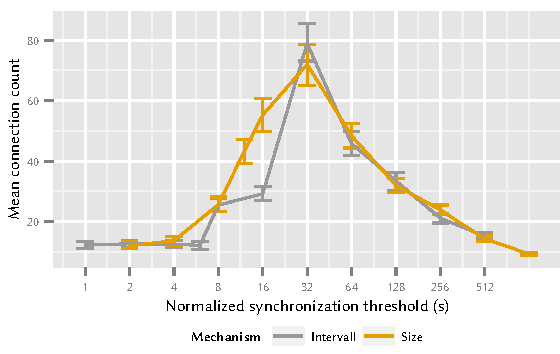
\includegraphics{application/cloud_file_synchronization/numerical_evaluation/figures/comparison}
  \caption{Comparison of algorithms with regard to normalized synchronization threshold \thresholdNormalised and connection count \connectionCount.}
  \label{fig:application:cloud_file_synchronisation:numerical_evaluation:mechanism_comparison:comparison}
\end{figure}

We observe that the mean connection count \connectionCount of both algorithms are interchangeable most of the time, as the interval length \thresholdInterval and the size threshold \thresholdSize can be converted into each other.
However, the results for a normalised synchronisation threshold \thresholdNormalised of \SI{16}{\second} vary significantly.
If we consider the \algointerval algorithm, the average amount of data transferred from the camera to the mobile client is \(\SI{16}{\second} \cdot \panTransferRate=\SI{8}{\mega\byte}\), which is uploaded in approximately \(\SI{8}{\mega\byte} / E[U] = \SI{1}{\second}\).
For the \algosize algorithm, the amount of data transferred from the camera to the mobile client has to accumulate to \SI{8}{\mega\byte} in order to result in a normalized synchronisation threshold \thresholdNormalised of \SI{16}{\second}.
Consequently, the mean upload time is also \SI{1}{\second}.
In conjunction with a disconnection timeout of \(\idleThreshold = \SI{11.576}{\second}\) it is likely that the connection is closed after the upload in both cases.

However, even if the mean upload times in both cases are equal, the variance of the upload time distributions vary.
The \algosize algorithm assures that always the same amount of data is uploaded, therefore the variance of the upload time distribution is only influenced by the variance of the upload bandwidth.
In the case of the \algointerval algorithm, the amount of uploaded data varies, due to the different image sizes.
Therefore, the variance of the upload time distribution in this case is dependent on the variance of the upload bandwidth and the variance of the image size.
This increased variance leads in some cases to longer upload times avoiding a disconnect between two upload batches.
However, this effect only comes into account if the sum of the upload time and the disconnection timeout is close to the inter-send interval.

The comparison of both algorithms indicate that similar results are reproducible with both of them.
However, the time based algorithm allows a better control of the number of disconnects during the synchronisation process, as the inter-send interval can be adapted to the disconnection timeout. 
In order to adapt the size based algorithms accordingly, additional knowledge of the file arrival process is required to estimate the interval length \thresholdInterval.
In the following, we only consider the \algointerval algorithm as it is easier to configure and also more intuitive for the end-user than the \algosize algorithm. 

\subsubsection*{Tradeoff Analysis for Considered Stakeholders}\label{sec:application:cloud_file_synchronisation:numerical_evaluation:trade_off_analysis}

After analysing the different objectives of the stakeholders individually, we now consider the tradeoff between these contradicting optimisation goals, the mean waiting time for the file synchronisation \sojournTime, the mean relative disconnected time \relativeDisconnectedTime, and the mean connection count \connectionCount.

\begin{figure*}
  \centering
  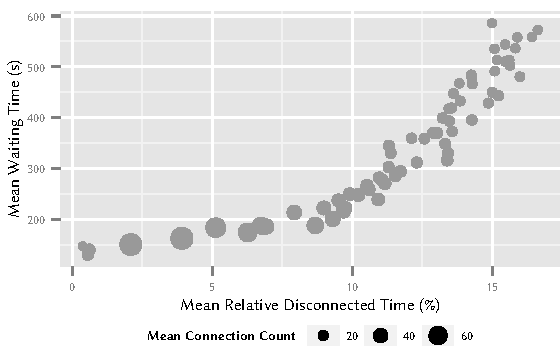
\includegraphics{application/cloud_file_synchronization/numerical_evaluation/figures/summary}
  \caption{Trade-off analysis of identified stakeholder objectives.}
  \label{fig:application:cloud_file_synchronisation:numerical_evaluation:trade_off_analysis:summary}
\end{figure*}

\reffig{fig:application:cloud_file_synchronisation:numerical_evaluation:trade_off_analysis:summary} depicts the mean waiting time for the file synchronisation on the y-axis and the mean relative disconnected time on the x-axis.
Each point in the figure corresponds to one parameter setting for the \algointerval, the size of the point depicts the mean connection count \connectionCount for this parameter setting.
For each stakeholder objective we have different optimisation goals.
While the user wants to minimise the mean waiting time \sojournTime of the file synchronisation, the user also is interested in maximising the mean relative disconnected time \relativeDisconnectedTime in order to save power.
The network provider wants to minimise the signalling overhead, thus the mean connection count \connectionCount should also be minimise.
Therefore, an optimal parameter set would be located on the right bottom of the figure, small mean waiting time and high relative disconnected time \relativeDisconnectedTime, and depicted by a small point indicating a small mean connection count \connectionCount.
However, the figure indicates that an increase in mean relative disconnected \relativeDisconnectedTime time also results in an increased mean waiting time \sojournTime.
We see that allowing for a small increase in waiting time \sojournTime of less than a minute can result in twice the time spent in disconnected state, i.e.\ additional power savings.
This change in metrics can be facilitated by increasing the inter-send interval length from \SI{32}{\second} to \SI{128}{\second} for the \algointerval algorithm.
An additional benefit of this change is a decrease of the connection count \relativeDisconnectedTime of more than \SI{50}{\percent}, resulting in a significantly reduced signalling load in the network.
